%%%%%%%%%%%%%%%%%%%%%%%%%%%%%%%%%%%%%%%%%
% Focus Beamer Presentation
% LaTeX Template
% Version 1.0 (8/8/18)
%
% This template has been downloaded from:
% http://www.LaTeXTemplates.com
%
% Original author:
% Pasquale Africa (https://github.com/elauksap/focus-beamertheme) with modifications by 
% Vel (vel@LaTeXTemplates.com)
%
% Template license:
% GNU GPL v3.0 License
%
% Important note:
% The bibliography/references need to be compiled with bibtex.
%
%%%%%%%%%%%%%%%%%%%%%%%%%%%%%%%%%%%%%%%%%

%----------------------------------------------------------------------------------------
%	PACKAGES AND OTHER DOCUMENT CONFIGURATIONS
%----------------------------------------------------------------------------------------

\documentclass{beamer}

\usetheme{focus} % Use the Focus theme supplied with the template
% Add option [numbering=none] to disable the footer progress bar
% Add option [numbering=fullbar] to show the footer progress bar as always full with a slide count

% Uncomment to enable the ice-blue theme
\definecolor{main}{RGB}{92, 138, 168}
\definecolor{background}{RGB}{240, 247, 255}

%------------------------------------------------

\usepackage{booktabs} % Required for better table rules

%----------------------------------------------------------------------------------------
%	 TITLE SLIDE
%----------------------------------------------------------------------------------------

\title{Wireless Communications \\Systems: \\ Lab session 1}

\subtitle{Digital modulations}

\author{Gilad Yair Nevo \\ Efi Dvir \\ Oren Zaharia}

\titlegraphic{
\includegraphics[scale=1.5]{Images/image1_.png}} % Optional title page image, comment this line to remove it

\institute{Communication Systems Engineering \\ Ben-Gurion University}

\date{Spring 2019}

%------------------------------------------------

\begin{document}

%------------------------------------------------

\begin{frame}
	\maketitle % Automatically created using the information in the commands above
\end{frame}

%----------------------------------------------------------------------------------------
%	 SECTION 1
%----------------------------------------------------------------------------------------

\section{Preliminary} % Section title slide, unnumbered

%------------------------------------------------

\begin{frame}{Digital Modulation}
	\begin{itemize}
	    \item PSK and ASK  are the simplest and basic digital modulations.
	    \item QPSK and QAM using the scheme of PSK and ASK.
	    \item CDMA - Code-division multiple access
        \item OFDM - Orthogonal frequency-division multiplexing 
	\end{itemize}
\end{frame}

%------------------------------------------------

\begin{frame}{CDMA}
\begin{itemize}
    \item A multiple access scheme where several users may share the same
physical medium (literally).
    \item The signals of the individual users are orthogonal.
    \item The information can be recovered without interference from other users.
    \item CDMA use pseudorandom sequences are approximately orthogonal to each other, that is they show good correlation properties.
    \item CDMA is based on spread spectrum,
that is, the spectral band is spread by multiplying the signal with such a pseudorandom
sequence.
\end{itemize}
\end{frame}
%------------------------------------------------
\begin{frame}{OFDM}
\begin{itemize}
    \item A digital multicarrier transmission technique.
    \item Digitally encoded symbols over several subcarrier frequencies.
    \item Clock rate to achieve robustness against long echoes in a multi-path radio channel.
    \item The information can be completely
    \item Mathematically, OFDM is a consequence of the orthogonality of the base functions of the Fourier series.
\end{itemize}
\end{frame}


%------------------------------------------------

%\begin{frame}[noframenumbering]{No Slide Numbering}
%	This slide is not numbered and is citing reference \cite{knuth74}.
%\end{frame}

%------------------------------------------------

\begin{frame}{Definitions}
\begin{itemize}
    \item Capacity: $C=B\log_{2}\left(1+\text{SINR}\right)$
    \item 
    \item 
    \item 
\end{itemize}
\end{frame}

%------------------------------------------------

\begin{frame}{Long Term Evolution}
Feature keys:
\begin{itemize}
    \item LTE was designed by a collaboration of national and regional telecommunications standards bodies known as the Third Generation Partnership Project (3GPP).
    \item The successor of the WCDMA, Known as the 4th generation of cellular.
    \item LTE is using \textbf{MIMO} technique (Multiple Inputs, Multiple Outpus).
    \item OSI Protocols are in use, each UE have an assigned IP address.
\end{itemize}
\end{frame}
%------------------------------------------------
\begin{frame}{LTE \\ System Architecture Evolution}
	\begin{block}{UE - User Equipment}
		The actual communication device is known as the mobile equipment (ME). In the
case of a voice mobile or a smartphone, this is just a single device.
	\end{block}
	\pause % Automatically creates a new "page" split between the above and above + below
	\begin{block}{EPC - Evolved Packet Core}
	    The "backbone" of the LTE network.
	\end{block}
	\pause % Automatically creates a new "page" split between the above and above + below
	\begin{block}{eNodeB - Evolved Node B}
		 eNB is a base station that controls the mobiles in one or more cells.
		 The base station that is communicating with a
mobile is known as its serving eNB.
	\end{block}
\end{frame}
%------------------------------------------------
\begin{frame}{UE - User Equipment}
\begin{itemize}
    \item UE
\end{itemize}
\end{frame}
%------------------------------------------------
%------------------------------------------------
\begin{frame}{EPC - Evolved Packet Core}
The EPC is assembled by many components
\begin{itemize}
    \item Home subscriber server (HSS).
    \pause
    \item Packet data network (PDN).
        \begin{itemize}
            \item Gateway (P-GW)
            \item The serving gateway (S-GW).
        \end{itemize}
    \pause
    \item The mobility management entity (MME) controls the high-level operation of the mobile.
    \pause
    \item Home subscriber server (HSS).
    \pause
    \item Home subscriber server (HSS).
\end{itemize}
\end{frame}
%------------------------------------------------
%------------------------------------------------
\begin{frame}{eNodeB - Evolved Node B}
Main functions:
\begin{itemize}
    \item The eNB sends radio transmissions to all its mobiles on the downlink and receives transmissions from them on the uplink, using the analogue and digital signal processing functions of the LTE \textbf{air interface}.
    \pause % Automatically creates a new "page" split between the above and above + below
    \item The eNB controls the low-level operation of all its mobiles, by sending them signalling messages such as \textbf{handover} commands that relate to those radio transmissions.
\end{itemize}
\end{frame}
%------------------------------------------------
\iffalse
\begin{frame}{Typesetting and Math}
	The packages \texttt{inputenc} and \texttt{FiraSans}\footnote{\url{https://fonts.google.com/specimen/Fira+Sans}}\textsuperscript{,}\footnote{\url{http://mozilla.github.io/Fira/}} are used to properly set the main fonts.
	\vfill
	This theme provides styling commands to typeset \emph{emphasized}, \alert{alerted}, \textbf{bold}, \textcolor{example}{example text}, \dots
	\vfill
	\texttt{FiraSans} also provides support for mathematical symbols:
	\begin{equation*}
		e^{i\pi} + 1 = 0.
	\end{equation*}
\end{frame}
\fi
%----------------------------------------------------------------------------------------
%	 SECTION 2
%----------------------------------------------------------------------------------------

\section{Practice}

%------------------------------------------------

\begin{frame}{Flowchart}
	\begin{block}{UE $\iff$ eNodeB Connection}
		\begin{itemize}
		    \item Power on procedure (next slide).
		    \item Wireshark
		\end{itemize}
	\end{block}
	\pause % Automatically creates a new "page" split between the above and above + below
	\begin{block}{Alert block}
		\begin{itemize}
		    \item Power Headroom reporting \\ A mobile's power headroom is the difference between its maximum transmit power and the power requested for its PUSCH transmission \iffalse LTE 10.1.4 page 162\fi.
		\end{itemize}
	\end{block}
	\pause % Automatically creates a new "page" split between the above and above + below
	\begin{exampleblock}{Example block}
		Example \textcolor{example}{text}.
	\end{exampleblock}
\end{frame}
%------------------------------------------------
%------------------------------------------------
\begin{frame}{Power On procedure}
    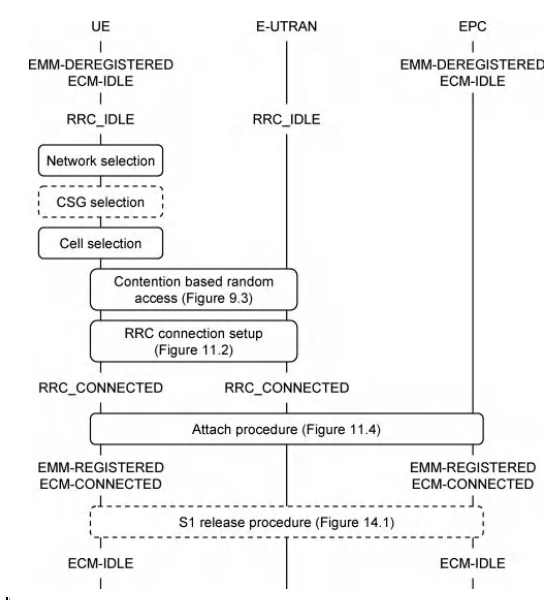
\includegraphics[width=\textwidth,height=\textheight,keepaspectratio]{power_on_sequence.png}

\end{frame}
%------------------------------------------------
\begin{frame}{Power On procedure}
On power on, the UE (user equipment) begins by running the procedure for network and cell selection, which has three steps.
    \begin{itemize}
        \item The mobile (UE) selects public land mobile network (PLMN).
        \item  The mobile can optionally ask the user to select a closed subscriber group (CSG) for registration. 
        \item The mobile selects a cell that belongs to the selected network and if necessary to the selected CSG.
    \end{itemize}
The mobile then contacts the corresponding base station using the contention based random access, and initiates the procedure for RRC connection establishment.
\\ RRC modes:
\begin{itemize}
    \item RRC\_IDLE 
    \item RRC\_CONNECTED
\end{itemize}
\end{frame}
%------------------------------------------------
\begin{frame}{Power On procedure}
    The final step, the mobile uses the attach procedure to contact the EPC (evolved packet core).\\ The UE accuires an IP address and established a tunnel to communicate out.
    \\\\
    
    The mobile is now in the states RRC\_CONNECTED, EMM\_REGISTERED and ECM\_CONNECTED. 
\end{frame}
%------------------------------------------------

\begin{frame}{Columns}
	\begin{columns}
		\column{0.5\textwidth}
			This text appears in the left column and wraps neatly with a margin between columns.
		
		\column{0.5\textwidth}
			
\includegraphics[width=\linewidth]{Images/placeholder.jpg}
	\end{columns}
\end{frame}

%------------------------------------------------

\begin{frame}{Lists}
	\begin{columns}[T, onlytextwidth] % T for top align, onlytextwidth to suppress the margin between columns
		\column{0.33\textwidth}
			Items:
			\begin{itemize}
				\item Item 1
				\begin{itemize}
					\item Subitem 1.1
					\item Subitem 1.2
				\end{itemize}
				\item Item 2
				\item Item 3
			\end{itemize}
		
		\column{0.33\textwidth}
			Enumerations:
			\begin{enumerate}
				\item First
				\item Second
				\begin{enumerate}
					\item Sub-first
					\item Sub-second
				\end{enumerate}
				\item Third
			\end{enumerate}
		
		\column{0.33\textwidth}
			Descriptions:
			\begin{description}
				\item[First] Yes.
				\item[Second] No.
			\end{description}
	\end{columns}
\end{frame}

%------------------------------------------------

\begin{frame}{Table}
	\begin{table}
		\centering % Centre the table on the slide
		\begin{tabular}{l c}
			\toprule
			Discipline & Avg. Salary \\
			\toprule
			\textbf{Engineering} & \textbf{\$66,521} \\
			Computer Sciences & \$60,005\\
			Mathematics and Sciences & \$61,867\\
			Business & \$56,720\\
			Humanities \& Social Sciences & \$56,669\\
			Agriculture and Natural Resources & \$53,565\\
			Communications & \$51,448\\
			\midrule
			\textbf{Average for All Disciplines} & \textbf{\$58,114}\\
			\bottomrule
		\end{tabular}
	\caption{Table caption}
	\end{table}
\end{frame}

%------------------------------------------------

\begin{frame}[focus]
	Thanks for using \textbf{Focus}!
\end{frame}

%----------------------------------------------------------------------------------------
%	 CLOSING/SUPPLEMENTARY SLIDES
%----------------------------------------------------------------------------------------

\appendix

\begin{frame}{References}
	\nocite{*} % Display all references regardless of if they were cited
	\bibliography{example.bib}
	\bibliographystyle{plain}
\end{frame}

%------------------------------------------------

\begin{frame}{Backup Slide}
	This is a backup slide, useful to include additional materials to answer questions from the audience.
	\vfill
	The package \texttt{appendixnumberbeamer} is used to refrain from numbering appendix slides.
\end{frame}

%----------------------------------------------------------------------------------------

\end{document}
